\documentclass[12pt]{article}
\usepackage{amsmath,amsfonts, epsfig}
\usepackage{booktabs} % for better table formatting
\usepackage{array}
\usepackage{multirow}
\usepackage{graphicx}
\usepackage{fancyhdr}
\usepackage{bm}
\pagestyle{fancy}
\lfoot{\texttt{ematm0067.github.io}}
\lhead{Introduction to AI - 03.2\_mlp - Conor}
\rhead{\thepage}
\cfoot{}

\usepackage{tikz}
\usetikzlibrary{positioning}

\usetikzlibrary{shapes.misc}


\usepackage{ifthen,calc}
\newboolean{nopics}
\setboolean{nopics}{false}


\begin{document}

\section*{A non-linear classifier.} 

Obviously one severe limitation of perceptron and other linear
classifiers is that it only works for problems that are in some sense
linear. There are lots of ways to try to address this, the
\textsl{kernel trick} for example does a non-linear transformation to
the data before running the classifier and relies, very roughly, on
the idea that in higher dimensions problems are more likely to be
linear. The approach we are going to look at is the neural
network\footnote{It is possible that neural networks are just a
complicated way of doing the kernel trick, that's not a discussion for
here though!}.

We can start with a simple insight from neuroscience; the perceptron
only has two layers, an input and an output, the brain is much more
complicated and the visual signal coming in to your eyes goes through
a series of successive sets of neurons before you decide you are now
reading the word `lion', or whatever. This makes you think it might be
a good idea to add more layers. In the simplest case that leads to a
multilayer perceptron or MLP. We will look first at how the MLP might
work to solve classification problems and then discuss how it might be
trained.

We will start with the simple case of a binary classification, so we
imagine the output gives the probability the input belongs to class
$a$, for simplicity the input will have three dimensions in the
diagram, of course it is easy to change this. The logistic classifier
we looked at before is something like
\begin{center}
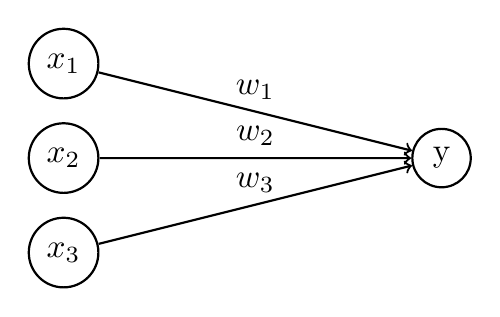
\begin{tikzpicture}[thick, scale=1.2, every node/.style={scale=1.2}]

% Input neurons
\foreach \i in {1,...,3} {
    \node[circle, draw, fill=white] (x\i) at (0,-\i) {$x_{\i}$};
}

% Output neuron
\node[circle, draw, fill=white] (output) at (4,-2) {y};

% Connections with weights
\foreach \i in {1,...,3} {
    \draw[->] (x\i) -- (output) node[midway, above] {$w_{\i}$};
}


\end{tikzpicture}
\end{center}
The idea is that this represents
\begin{equation}
  y=\phi(\sum_j w_j x_j + b)
\end{equation}
where $\phi$ in this case will be the logistic function:
$\phi(r)=\sigma(r)$ and the parameters are $\theta=(w_1,w_2,b)$, in
this context the $w$s are called \textsl{weights} and the $b$ is a
\textsl{bias}. Now $y$ is a function of the input
$\mathbf{x}=(x_1,x_2)$: you could write $y(\mathbf{x};\theta)$ where
the semi-colon is seperating the variables, which are different for
each data point and the parameters, which are adjusted during
learning. We have seen to make $y(\mathbf{x})$ as close as possible to
$p(a)$, but, as we keep saying, this assumes that this mapping, from
data values to probability, can be sensibly done using a linear
function.

An MLP, inspired by the brain, fixes this by adding more layers, here
is what it would look like with one extra \textsl{hidden} layer.
\begin{center}
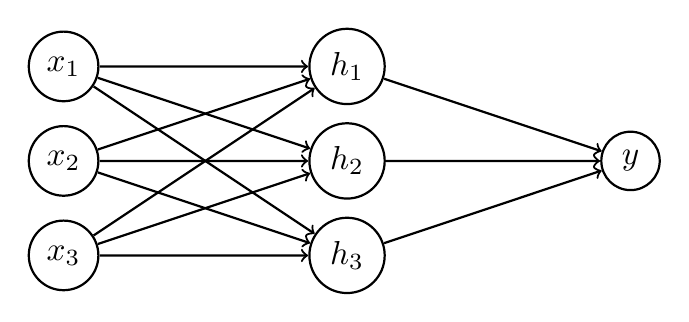
\begin{tikzpicture}[thick, scale=1.2, every node/.style={scale=1.2}]

% Input neurons
\foreach \i in {1,...,3} {
    \node[circle, draw, fill=white] (x\i) at (0,-\i) {$x_{\i}$};
}

% Hidden layer neurons
\foreach \i in {1,...,3} {
    \node[circle, draw, fill=white] (h\i) at (3,-\i) {$h_{\i}$};
}

% Output neuron
\node[circle, draw, fill=white] (output) at (6,-2) {$y$};

% Connections from inputs to hidden layer
\foreach \i in {1,...,3} {
    \foreach \j in {1,...,3} {
        \draw[->] (x\i) -- (h\j);
    }
}

% Connections from hidden layer to output
\foreach \i in {1,...,3} {
    \draw[->] (h\i) -- (output);
}

\end{tikzpicture}
\end{center}
Now the function is more complicated, we have
\begin{equation}
  h_i=\phi(\sum_j w^1_{ij}x_j+b^1_i)
\end{equation}
and, almost as before
\begin{equation}
  y=\sigma(\sum_j w^2_j h_j+b^2)
\end{equation}
where, since we want $y$ to be a probability, we continue to use a logistic function for the activation. We have a wider choice for $\phi(r)$, a common choice is the ReLU:
\begin{equation}
  \phi(r)=\left\{\begin{array}{ll}r&r\ge 0\\0&\text{otherwise}\end{array}\right.
\end{equation}
Why this is a good choice is complicated, it is easy to suggest it has
nice properties, but lots of different possibities have other, similar
or competing, nice properties and so, for now, the answer is that it
seems to work well and robustly.

As a sort of aside, we can write this in matrix form:
\begin{equation}
  \mathbf{h}=\phi.(W^1 \mathbf{x}+\mathbf{b})
\end{equation}
and 
\begin{equation}
  y=\sigma.(\mathbf{w}\cdot\mathbf{h}+b^2)
\end{equation}
I have used the `broadcast' notation from Julia, if $f:\textbf{R}\rightarrow\textbf{R}$ is a function defined on scalars then we lift this to a function on vectors componentwise:
\begin{equation}
  f.(\textbf{x})=[f(x_1),f(x_2),\ldots,f(x_n)
\end{equation}
Mostly this is just me being annoying since I spent time with people who worry too much about notation, most people don't bother with the dot; it is important not to get too hung up on notation, but also not to be too lazy about it either!

The main thing is we still have a function $y(\mathbf{x};\theta)$ but
it is a much more complicated function and has lots more parameters
\begin{equation}
  \theta=(W^1,\mathbf{b}^2,\mathbf{w}^2,b)
\end{equation}
In the example here it has, without worrying too much about
independence, 9+3+3+1=16 parameters when the perceptron has only
four. The hope is that this allows a much richer classification and
the straight line or hyperplane is replaced by something more
complicated.

As a simple example lets try to classify points in two dimensions, the
$b$ points are more than $r=1$ from the center, the $a$ are
less. This would not be possible with a linear classifier and so I tried this
\begin{center}
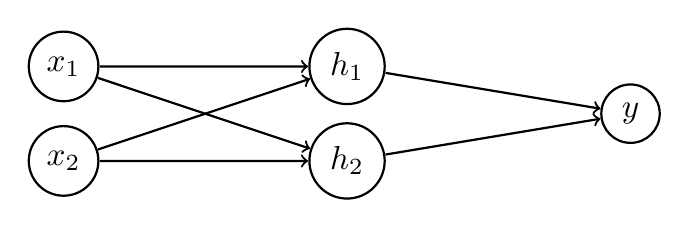
\begin{tikzpicture}[thick, scale=1.2, every node/.style={scale=1.2}]

% Input neurons
\foreach \i in {1,...,2} {
    \node[circle, draw, fill=white] (x\i) at (0,-\i) {$x_{\i}$};
}

% Hidden layer neurons
\foreach \i in {1,...,2} {
    \node[circle, draw, fill=white] (h\i) at (3,-\i) {$h_{\i}$};
}

% Output neuron
\node[circle, draw, fill=white] (output) at (6,-1.5) {$y$};

% Connections from inputs to hidden layer
\foreach \i in {1,...,2} {
    \foreach \j in {1,...,2} {
        \draw[->] (x\i) -- (h\j);
    }
}

% Connections from hidden layer to output
\foreach \i in {1,...,2} {
    \draw[->] (h\i) -- (output);
}

\end{tikzpicture}
\end{center}
with 400 points, half red and half blue. It didn't seem to work either, the functions it could produce weren't complicated enough, so I expanded the network further to this:
\begin{center}
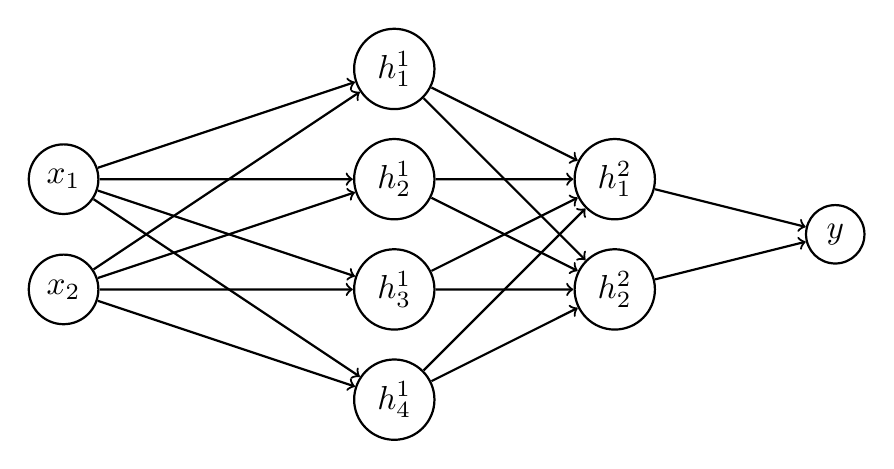
\begin{tikzpicture}[thick, scale=1.4, every node/.style={scale=1.2}]

% Input neurons
\foreach \i in {1,...,2} {
    \node[circle, draw, fill=white] (x\i) at (0,-\i) {$x_{\i}$};
}

% First hidden layer neurons
\foreach \i in {1,...,4} {
    \node[circle, draw, fill=white] (h1_\i) at (3,1-\i) {$h^1_{\i}$};
}

% Second hidden layer neurons
\foreach \i in {1,...,2} {
    \node[circle, draw, fill=white] (h2_\i) at (5,-\i) {$h^2_{\i}$};
}

% Output neuron
\node[circle, draw, fill=white] (output) at (7,-1.5) {$y$};

% Connections from inputs to first hidden layer
\foreach \i in {1,...,2} {
    \foreach \j in {1,...,4} {
        \draw[->] (x\i) -- (h1_\j);
    }
}

% Connections from first to second hidden layer
\foreach \i in {1,...,4} {
    \foreach \j in {1,...,2} {
        \draw[->] (h1_\i) -- (h2_\j);
    }
}

% Connections from second hidden layer to output
\foreach \i in {1,...,2} {
    \draw[->] (h2_\i) -- (output);
}


\end{tikzpicture}
\end{center}
The two hidden layers use a ReLU activation.

With this MLP, with two hidden layers, the classifier works, in
Fig.~\ref{fig:mlp} I have plotted $y$, the estimated probability that a point is
from the $a$ class, as a function of position. In other words I
randomly produce 200 points whose distance from the center is less
than one, the $a$ points, and another 200 points where the distance is
greater than one, the $b$ points. I train the neural network to
classify these points, with $y$ near one corresponding to an $a$
point, by training the neural network I mean fixing the values of the
parameters $\theta$, in this case this is all the weights for the
links from the input to the first hidden layer, $2\times 4=8$ of
these, the biases for the first hidden layer, the weights between the
hidden layers, the biases for the second hidden layer and, finally,
the weights from the second hidden layer to the output and the bias
for the output. This makes $8+4+8+2+2+1=25$ parameters in all. How I
fix these values is the subject of the next note! Finally, to make the
picture I plot a heatmap for the map from $\textbf{x}$, the input, to
$\textbf{y}$, the output. As you can see it is a pretty good
approximation of the circle.

\begin{figure}[thb]
\begin{center}
  \includegraphics[width=0.8\textwidth]{two_layer_heatmap.png}
\end{center}
\caption{The estimated probability of a point belonging to class $a$
  using the MLP with two hidden layers, what could be called a
  $2\times 4\times 2\times 1$ MLP since the layers have sizes two for
  the input, four for the first hidden layer, two for the second and
  one for the output. The $a$ points all lie in the circle of radius
  one and it is clear the MLP has approximated this decision boundary
  with a hexagon. The code is available in the github and if you play
  with it you'll see that increasing the number of points will give a
  more regular hexagon.}\label{fig:mlp}
\end{figure}

It is interesting to experiment with the number and size of the
layers; these numbers which aren't fixed by training are often called
\textsl{meta-parameters}. A $2\times 8 \times 4\times 2\times 1$ MLP,
for example, with three hidden layers, gives a rounder decision boundary and the $2\times 8  \times 4\times 4\times 2\times 1$ MLP gives a very crisp decision boundary. This is shown in Fig.~\ref{fig:mlp_bigger}.


\begin{figure}[thb]
  $$
    \begin{array}{ll}
      \textbf{A}&\textbf{B}\\
      \includegraphics[width=0.4\textwidth]{two_layer_heatmap_842.png}&
      \includegraphics[width=0.4\textwidth]{two_layer_heatmap_8442.png}
    \end{array}
    $$
\caption{The estimated probability of a point belonging to class $a$
  using more complicated MLP, in \textbf{A} with three hidden layers giving a 
  $2\times 8\times 4\times 2\times 1$ and in \textbf{B} with four hidden layers giving $2\times 8\times 4\times 4\times 2\times 1$.}\label{fig:mlp_bigger}
\end{figure}

\subsection*{More than two classes}

So far we have looked at examples with just two classes and have used
an MLP with a single output neuron, with a high input associated with
one class and low with the other. Obviously this is not ideal; we'd
like more than one class. The way to do this is to have an output node
for each class:
\begin{equation}
  y_i = \sum w_{ij} h_j +b_i
\end{equation}
where the $h_j$ is supposed to represent the preceeding hidden layer,
in practice of course there will usually be more than one hidden layer
so there might be other indices or labels on the various variable. Now
you will notice that this is a linear layer. We do want to use an
activation function to convert the $y_i$s into probabilities so that
we go from $y_i$ to $p_i$, the estimated probability that the input
corresponds to the $i$th class. However, these probabilities must add to one:
\begin{equation}
  p_1+p_2+\ldots+p_c=1
\end{equation}
where there are $c$ classes. This means that the non-linearity applied to specific $y_i$ must involve all the $y_i$s at once. The usual solution to this complication is to use the \textsl{softmax} function:
\begin{equation}
  p_i=\sigma(\mathbf{y})_i=\frac{e^{y_i}}{\sum_j e^{y_j}}
\end{equation}
It is easy to see that this gives values between zero and one and that
the probabilities add to one.

We will look at all this more in the next set of notes when we
consider training, but for now lets look at an example, in
Fig.~\ref{fig:three_class} we see the $p_i$ in an example with a
two-dimensional input and three classes; for it to work, that is for
the MLP to be able to learn the decision boundaries, a rather large
MLP is used: $2\times 16\times 8\times 4\times 3$, but with this architecture it succeeds.



\begin{figure}[thb]
  $$
    \begin{array}{lll}
      \textbf{A}&\textbf{B}&\textbf{C}\\
      \includegraphics[width=0.3\textwidth]{heatmap_class_0.png}&
      \includegraphics[width=0.3\textwidth]{heatmap_class_1.png}&
      \includegraphics[width=0.3\textwidth]{heatmap_class_2.png}
    \end{array}
    $$
\caption{The estimated probability of a point belonging to class each of three classes, with \textbf{A}, \textbf{B} and \textbf{C} each corresponding to one class. Here the input is two-dimensional, points in the first class are all inside a unit circle, the second class has points outside the circle with $x_2>0$ and the third class has points outside the circle but with $x_2<0$, For training there were 160 of each point type.}\label{fig:three_class}
\end{figure}

Obviously we haven't looked at training yet, that comes next. Another
thing to note is that we have only used data sets where there are no
`difficult' points, outliers, or mistakes or just odd twists and turns
in the decision boundary; the ability of neural networks to deal
reasonably well with this sort of problem is part of what makes them
so effective.


\end{document}

